\documentclass{article}

\usepackage[dutch]{babel}
\usepackage[margin=3cm]{geometry}
\usepackage{graphicx}
\usepackage{float}
\usepackage{caption}
\usepackage{hyperref}
\usepackage{amsmath}
\usepackage{wrapfig}
\usepackage[parfill]{parskip}

% fonts
\usepackage[T1]{fontenc}
\usepackage{helvet}
\renewcommand{\familydefault}{\sfdefault}

\graphicspath{{img/}}

% theorem environment
\usepackage{amssymb}

\newtheorem{theorem}{Definitie}[section]

\usepackage{enumitem}

\newenvironment{thmenum}
 {\begin{enumerate}[label=\upshape\bfseries(\roman*)]}
 {\end{enumerate}}

\usepackage{minted}
\setminted{frame=single,framesep=3pt,linenos}
\usepackage{upquote}
\usepackage{color}

\begin{document}

\begin{titlepage}
    \author{Tuur Vanhoutte}
    \title{Backend Development}
\end{titlepage}

\pagenumbering{gobble}
\maketitle
\newpage
\tableofcontents
\newpage

\pagenumbering{arabic}

\section{.Net Core \& Web API}

\subsection{.NET Historiek}

\subsubsection{.NET Framework}

\begin{itemize}
    \item Ontwikkeling .NET Framework \& C\# begonnen einde Jaren 90 (Opkomst van Java, Microsoft moest reageren $\Rightarrow$ C\#)
    \item Versie 1.0 .NET Framework op 13 February 2002
    \item Windows Only
    \begin{itemize}
        \item Beperkt open source via Home | Mono (\url{mono-project.com})
    \end{itemize}
    \item Was vooral framework voor desktop applicaties (Winforms, WPF)
    \item Web applicaties via ASP.NET Forms
    \item Laatste versie .NET Framework is 4.8 (april 2019)
    \item Geen verdere ontwikkeling meer van .NET Framework
\end{itemize}

\subsubsection{Rond 2012 enkel strategische veranderingen}

\begin{itemize}
    \item Dominantie Windows was minder groot geworden
    \begin{itemize}
        \item Opkomst mobile devices (iPhone, Android)
        \item Cloud was belangrijker aan het worden (veel Linux)
        \item Open-source werd belangrijker
    \end{itemize}
    \item Microsoft zag een shift van .NET Framework naar andere technologie (Node, Python, etc\dots)
\end{itemize}

\subsubsection{Ontwikkeling .NET Core}

\begin{itemize}
    \item Cross platform (Windows/Linux/macOS)
    \item Volledig open-source
    \begin{itemize}
        \item Samsung TV
        \item ARM Raspberry Pi
        \item \dots
    \end{itemize}
    \item Clean-up van bestaande .NET Framework code
    \item Zoveel mogelijk compatibel
    \item Built for the Cloud
\end{itemize}

Sinds November 2020 spreken we niet meer over .NET Framework of .NET Core maar over .NET 5, .NET 6, .NET 7, \dots

\subsubsection{Tijdslijn}

\begin{itemize}
    \item .NET 5 $\Rightarrow$ November 2020
    \item .NET 6 $\Rightarrow$ November 2021 (LTS)
    \item .NET 7 $\Rightarrow$ November 2022
    \item .NET 8 $\Rightarrow$ November 2023 (LTS)
    \item LTS $\Rightarrow$ 3 jaar support
    \item Zonder LTS $\Rightarrow$ 1 jaar support
\end{itemize}

Alles volledig opensource via \url{https://github.com/dotnet}

\subsection{Soorten .NET applicaties}

\subsubsection{Type applicaties in .NET 5:}

\begin{itemize}
    \item ASP.NET Web Applicaties
    \item Console Applicaties
    \item Xamarin
    \item Winforms \& WPF Desktop applicaties
\end{itemize}

\subsubsection{Ondersteuning voor verschillende talen}

\begin{itemize}
    \item C\# (wij gebruiken dit)
    \item Visual Basic
    \item F\# (functional programming)
    \item C++ (desktop development)
\end{itemize}

\subsubsection{Toekomst desktop development}

\begin{itemize}
    \item Zeker nog belangrijk
    \item Niet alles kan in de browser (vb zware 3D apps, interfacing met machines etc)
    \item Zit niet meer in MCT opleiding (wel Xamarin natuurlijk)
    \item Project MAUI
    \begin{itemize}
        \item 1 framework voor .NET/Xamarin/Windows Desktop
        \item Introducing .NET Multi-platform App UI | .NET Blog : \url{https://devblogs.microsoft.com/dotnet/introducing-net-multi-platform-app-ui/}
    \end{itemize}
\end{itemize}

\subsection{ASP.NET Core}

= Framework voor het bouwen van Web Applicaties

\subsubsection{Verschillende soorten applicaties zijn mogelijk:}

\begin{itemize}
    \item Klassieke server-side framework (Razor) (zoals PHP,...)
    \item Realtime Framework (web sockets etc...) met als naam Signal R
    \item Frontend Framework Blazor (C\# in de browser)
    \begin{itemize}
        \item Web Assembly support
    \end{itemize}
    \item \textbf{Framework om API’s te bouwen , webapi (wij gebruiken dit)}
\end{itemize}

Cross platform zowel om uit te voeren als te onwikkelen (Visual Studio \& Visual Studio Code zijn cross-platform)

\subsubsection{ASP.NET Web API}

= Framework voor het bouwen van API’s voor toepassingen

Deze toepassingen zijn:

\begin{itemize}
    \item Front-End Web App (Vue, Angular, Blazor,...)
    \item Desktop Applications
    \item Alles wat HTTP calls kan uitvoeren en JSON begrijpt
\end{itemize}

Zelfde als HTTP Triggers in Azure Functions (cfr. Module IoT Cloud Semester 3)

\subsection{HTTP (Herhaling)}

= Hyper Tekst Transfer Protocol

\begin{itemize}
    \item Onderliggende protocol waarop Internet werkt
    \item Opvragen van tekst, bestanden vanaf servers
    \item Request \textit{meestal} afkomstig van een webbrowser maar ook smartphone, IoT device
    \item HTTP zal bepalen hoe een request en response er moeten uitzien
    \item HTTP bevat een aantal commando’s (HTTP Verbs)
    \item HTTP is stateless, het zal dus geen rekening houden met voorgaande requests
    \item HTTP is niet sessionless, we kunnen cookies (client-side) gebruiken om data bij te houden
    \item HTTP is relatief eenvoudig
\end{itemize}

\subsection{API Design}

\begin{itemize}
    \item In deze module gaan we API's programmeren
    \item De bedoeling is dat frontend applications deze gebruiken
    \item Onze API's zullen enkel JSON data ontvangen en terugsturen
    \item Oudere API's systemen keren soms ook XML terug (deze zien wij niet)
    \item Een API noemen we ook soms een endpoint
    \item De vorm en naamgeving is hier belangrijk
\end{itemize}

\subsubsection{Richtlijnen bij het opstellen van API URL's}

\begin{itemize}
    \item Gebruik Engelse woorden
    \item Start met het woord `api':
    \begin{itemize}
        \item http://www.mct.be/\textcolor{red}{api}
    \end{itemize}
    \item In de URL plaatsen we de naam van objecten die we wensen op te halen
    \begin{itemize}
        \item http://www.mct.be/api/\textcolor{red}{courses}
    \end{itemize}
    \item Willen we specieke cursus ophalen op basis van zijn code steken we dit in de URL
    \begin{itemize}
        \item http://www.mct/be/api/courses/\textcolor{red}{MCT2IOTCLOUD}
    \end{itemize}
    \item Willen we de weken ophalen, plaatsen we dit ook in de URL
    \begin{itemize}
        \item http://www.mct/be/api/courses/MCT2IOTCLOUD/\textcolor{red}{weeks}
    \end{itemize}
    \item Zoeken in de weken kunnen we als volgt gaan doen:
    \begin{itemize}
        \item http://www.mct/be/api/courses/MCT2IOTCLOUD/weeks\textcolor{red}{?q=iothub}
    \end{itemize}
    \item Wil je een bepaalde week ophalen:
    \begin{itemize}
        \item http://www.mct/be/api/courses/MCT2IOTCLOUD/weeks/\textcolor{red}{1}
    \end{itemize}
    \item Wil je de docent ophalen kan dit op deze manier in de URL:
    \begin{itemize}
        \item http://www.mct/be/api/courses/MCT2IOTCLOUD/weeks/1/\textcolor{red}{teacher}
    \end{itemize}
\end{itemize}

\subsection{Anatomie van een ASP.NET Web API Project}

\subsubsection{csproj file}

\begin{figure}[H]
    \centering
    \includegraphics[width=0.5\textwidth]{csproj.png}
    \caption{csproj voorbeeld}
\end{figure}

\begin{itemize}
    \item Beschrijft project
    \item Zal ingelezen worden door Visual Studio
    \item Bevat alle referenties naar gebruikte nuget packages
    \item dotnet build etc zal deze file gebruiken
    \item We mogen deze wijzigen (maar weet wat je doet)
\end{itemize}



\subsubsection{Program.cs}

\begin{itemize}
    \item Main entry point van ASP.NET API applicatie
    \item Hier begint alles
    \item Soms moeten we hier iets instellen
    \item Voorlopig niet van belang
\end{itemize}

\subsubsection{Startup.cs}

\begin{itemize}
    \item Naam spreekt voor zich, bevat alle startup code voor onze API
    \item Hier bepalen we welke \textbf{services} we wensen te gebruiken van ASP.NET 
        
        
\end{itemize}

\begin{figure}[H]
    \centering
    \includegraphics[width=0.7\textwidth]{startup-cs1.png}
    \caption{ConfigureServices}
\end{figure}
\begin{figure}[H]
    \centering
    \includegraphics[width=0.4\textwidth]{startup-cs2.png}
    \caption{Controllers}
\end{figure}
\begin{figure}[H]
    \centering
    \includegraphics[width=0.6\textwidth]{startup-cs3.png}
    \caption{Swagger}
\end{figure}

\begin{theorem}[Dependency Injection]

Dependency Injection is het injecteren van services in de ASP.NET Container

(komen we later nog op terug)
\end{theorem}

\begin{figure}[H]
    \centering
    \includegraphics[width=0.7\textwidth]{startup-cs4.png}
    \caption{Configureren van de HTTP Pipeline}
\end{figure}
\begin{figure}[H]
    \centering
    \includegraphics[width=0.6\textwidth]{startup-cs5.png}
    \caption{Configureren van services}
\end{figure}
\begin{figure}[H]
    \centering
    \includegraphics[width=0.3\textwidth]{startup-cs6.png}
    \caption{Configureren van Routing, Security etc\dots}
\end{figure}


\textbf{HTTP Pipeline}

\begin{itemize}
    \item We spreken van middleware componenten in de pipeline
    \item Deze componenten zijn verbonden en geven de data door aan elkaar
    \item Ieder component zal zijn bijdrage leveren
    \item Endpoint is onze code in de controller
    \item Request en Response gaan door deze pipeline
    \item ASP.NET Core Middleware: \url{https://docs.microsoft.com/en-us/aspnet/core/fundamentals/middleware/?view=aspnetcore-5.0}
\end{itemize}

\begin{figure}[H]
    \centering
    \includegraphics[width=0.7\textwidth]{http-pipeline.png}
    \caption{De HTTP Pipeline met middleware componenten}
\end{figure}

\subsubsection{Appsetting.json}

= Configuratie info nodig in de applicatie

\begin{itemize}
    \item Niet inchecken in GitHub (.gitignore gebruiken)
    \item Bv.: Mailserver settings, connectionstrings etc...
    \item We zien later (in een labo) hoe we deze kunnen uitlezen
    \item We kunnen verschillende files gebruiken:
    \begin{itemize}
        \item Appsettings.Development.json
        \item Appsettings.Production.json
        \item \dots
    \end{itemize}
    \item Configuration in ASP.NET Core: \url{https://docs.microsoft.com/en-us/aspnet/core/fundamentals/configuration/?view=aspnetcore-5.0}
\end{itemize}

\subsection{Controllers}

\begin{itemize}
    \item Belangrijkste concept in ASP.NET
    \item Zorgt voor de verwerking van de requests
    \item Zal een response terugkeren naar de aanvrager (bv. onze React JS applicatie)
    \item Is klasse in map \textbf{Controllers} in onze applicatie
    \item Naam moet eindigen op \textbf{Controller}
    \item Klasse moet erven van \textbf{ControllerBase}
    \item Attribute [ApiController] moet er staan om aan te duiden dat het een API is als we [Route] gebruiken op Controller niveau
    \item Via [Route] kunnen we de URL bepalen
\end{itemize}

\begin{figure}[H]
    \centering
    \includegraphics[width=0.5\textwidth]{controller.png}
    \caption{Voorbeeld Controller}
\end{figure}


\subsubsection{Endpoints}

Controller bevat Endpoints = functies die we uitvoeren

\begin{itemize}
    \item Endpoint bevat HTTP Verb
    \begin{itemize}
        \item GET
        \item POST
        \item PUT
    \end{itemize}
    \item Endpoints voeren de code uit
    \begin{itemize}
        \item Data ophalen of toevoegen
        \item Berekening doen
        \item \dots
    \end{itemize}
\end{itemize}

\begin{figure}[H]
    \centering
    \includegraphics[width=0.5\textwidth]{controller-endpoint.png}
    \includegraphics[width=0.4\textwidth]{controller-endpoint2.png}
    \caption{HTTP GET \& POST}
\end{figure}

\textbf{Route}

\begin{itemize}
    \item Een route is de URL naar het Endpoint
    \item Er zijn verschillende routes mogelijk per Endpoint
    \item Dezelfde routes zijn mogelijk zolang het HTTP Verb verschillend is
    \item We kunnen parameters megeven in de route via \{\}
    \item Indien geen routes: Default is GET met route = naam van Controller
\end{itemize}

\begin{figure}[H]
    \centering
    \includegraphics[width=0.45\textwidth]{controller-routes.png}
    \includegraphics[width=0.5\textwidth]{controller-routes2.png}
    \caption{Meerdere routes per endpoint mogelijk (links). Delete request met parameters (rechts)}
\end{figure}

\begin{figure}[H]
    \centering
    \includegraphics[width=0.5\textwidth]{controller-voorbeeld.png}
    \caption{\underline{https://localhost:5001/wine/wines} en \underline{https://localhost:5001/wine/wijnen}}
\end{figure}

\begin{figure}[H]
    \centering
    \includegraphics[width=0.4\textwidth]{controller-routes4.png}
    \caption{/wine haalt hij uit de naam WineController}
\end{figure}

\begin{figure}[H]
    \centering
    \includegraphics[width=0.5\textwidth]{controller-routes-api.png}
    \caption{Best practice: met api in de naam}
\end{figure}

\begin{figure}[H]
    \centering
    \includegraphics[width=0.5\textwidth]{controller-routes-parameter.png}
    \caption{Route met parameter. https://localhost:5001/api/wines/\textcolor{red}{2005}}
\end{figure}

\begin{itemize}
    \item Endpoints keren altijd iets terug:
    \begin{itemize}
        \item Status codes
        \item Data die we opvragen
    \end{itemize}
    \item Niet altijd makkelijk wat je moet kiezen
    \item Status codes uit HTTP standaard 5 grote verdelingen
\end{itemize}

\begin{figure}[H]
    \centering
    \includegraphics[width=0.5\textwidth]{http-statuscodes.png}
    \caption{Status codes}
\end{figure}

Overzicht statuscodes: \url{https://restfulapi.net/http-status-codes/}

Meest gebruikt: 

\begin{itemize}
    \item 200 OK
    \item 201 Created
    \item 400 Bad Request, 401 Unauthorized, 403 Forbidden, 415 Unsupported Media Type
    \item 500 Internal Server Error
\end{itemize}

\textbf{Returnen van data en statuscodes: veel ingebouwde klassen}

\begin{itemize}
    \item OkObjectResult(data)
    \item Ok()
    \item NotFoundObjectResult(data)
    \item NotFound()
    \item StatusCodeResult(int statuscode)
\end{itemize}

\subsection{Model binding}

\begin{itemize}
    \item Default enkel bij HTTP Post $\Rightarrow$
    \item ASP.NET Core volgorde voor ophalen van key/values:
    \begin{itemize}
        \item Form fields
        \item Request body (enkel bij gebruik [ApiController] attribuut)
        \item Route
        \item Querystring
    \end{itemize}
\end{itemize}

\subsubsection{Voorbeelden}

\begin{figure}[H]
    \centering
    \includegraphics[width=0.5\textwidth]{model-binding-formfields.png}
    \caption{Voorbeeld: Form Fields}
\end{figure}

\begin{figure}[H]
    \centering
    \includegraphics[width=0.5\textwidth]{model-binding-requestbody.png}
    \caption{Voorbeeld: Request Body (enkel bij gebruik van [ApiController] attribuut)}
\end{figure}

Via Route attribuut kunnen we parameters doorgeven:

\begin{figure}[H]
    \centering
    \includegraphics[width=0.5\textwidth]{model-binding-parameter.png}
    \caption{We bepalen de parameter namen tussen de \{parameter naam\}}
\end{figure}

\begin{figure}[H]
    \centering
    \includegraphics[width=0.5\textwidth]{model-binding-parameter2.png}
    \caption{In de C\# functie voorzien we dezelfde naam als in de route}
\end{figure}

\begin{figure}[H]
    \centering
    \includegraphics[width=0.5\textwidth]{model-binding-parameter3.png}
    \caption{We kunnen ook de waarden uit de route direct opslaan in het object: via \textbf{[FromRoute]} attribuut}
\end{figure}

\begin{figure}[H]
    \centering
    \includegraphics[width=0.5\textwidth]{model-binding-querystring.png}
    \caption{Kan ook via Querystring}
\end{figure}

\subsection{Configuration}

\begin{itemize}
    \item Bepaalde info willen we niet hardcoden
    \begin{itemize}
        \item Mailserver, connectionstring, password, \dots
    \end{itemize}
    \item We moeten dit buiten de applicatie kunnen opslaan (appsettings.json, Azure Keyvault)
\end{itemize}

\subsubsection{appsettings.json}

\begin{itemize}
    \item JSON file die bij de applicatie zit
    \item Verschillende versies mogelijk
    \begin{itemize}
        \item Development/Testing/Production..
    \end{itemize}
    \item Eerst geladen
    \item Bevat dingen die zowel voor development als production geldig zijn
    \item appsettings.Development.json (naargelang de omgeving inladen)
    \begin{itemize}
        \item Overriden wat reeds in appsettings.json szit
    \end{itemize}
    \item JSON file
\end{itemize}

\begin{figure}[H]
    \centering
    \includegraphics[width=0.5\textwidth]{appsettings-json.png}
    \caption{Probeer met Secties te werken (zie MailServerSettings)}
\end{figure}

\begin{itemize}
    \item We gebruiken Option pattern voor inladen data uit configuratie files
    \item Eerst klasse maken die overeenkomt met de waarden in de JSON file
\end{itemize}

\begin{figure}[H]
    \centering
    \includegraphics[width=0.5\textwidth]{appsettings-json-secties.png}
    \caption{Klasse die overeenkomt met het MailServerSettings object in appsettings.json}
\end{figure}

\begin{itemize}
    \item Registreren van de sectie in de startup en koppelen aan de klasse
    \item Hierdoor krijgen we een strongly typed settings file
\end{itemize}

\begin{figure}[H]
    \centering
    \includegraphics[width=0.6\textwidth]{appsettings-json-configure.png}
    \caption{Configuration.GetSection("SectionNaam")}
\end{figure}

Gebruik in de controller: 

\begin{itemize}
    \item IOptions<MailServerSettings> via CONSTRUCTOR (CTOR) binnenbrengen
    \item Value property zal deze uitlezen en opslaan in property \_mailserverSettings
    \item Hierdoor kunnen we deze vlot uitlezen in de controller en gebruiken
\end{itemize}

\begin{figure}[H]
    \centering
    \includegraphics[width=0.5\textwidth]{appsettings-json-controller.png}
    \caption{}
\end{figure}

In VSCode:

\begin{itemize}
    \item launch.json openen
    \item Hier kan je de profielen vinden
    \item Copy/paste profile
    \item Per profiel kan je instellingen maken zoals URL of ASPNETCORE\_ENVIRONMENT
\end{itemize}

\begin{figure}[H]
    \centering
    \includegraphics[width=0.3\textwidth]{appsettings-json-vscode.png}
    \caption{launch.json}
\end{figure}

\begin{figure}[H]
    \centering
    \includegraphics[width=0.3\textwidth]{appsettings-json-vscode2.png}
    \caption{In de dropdown kies je wat je wil starten}
\end{figure}


\textbf{Visual Studio 2019}

\begin{itemize}
    \item We bepalen de profielen in de map Properties
    \item In launchSettings.json
\end{itemize}

\subsubsection{Azure Keyvault}

\begin{itemize}
    \item Kluis in Azure waar alle info zit
    \item Beste oplossing voor productie projecten
\end{itemize}

\subsection{Wat moet je kennen?}

\begin{itemize}
    \item Zorg dat je de HTTP Request/Response kan uitleggen
    \item Wat zijn statuscodes en wanneer gebruik ik welke
    \item Een duidelijke API URL kunnen opstellen
    \item Manieren van modelbinding
    \item Hoe configureer je uw omgeving met profielen
\end{itemize}

\section{Web API DTO, Validation, Versioning}

\subsection{Validation}




\begin{itemize}
    \item Altijd valideren:
    \begin{itemize}
        \item In client applicatie (Xamarin, React, Vue, Angular)
        \item In de backend
    \end{itemize}
    \item We gaan er altijd vanuit dat de binnenkomende data foutief of ongeldig kan zijn
    \item Vertrouw niemand
    \item WebAPI bevat ingebouwd systeem om validatie te doen
\end{itemize}

\subsubsection{Attributen}

\begin{figure}[H]
    \centering
    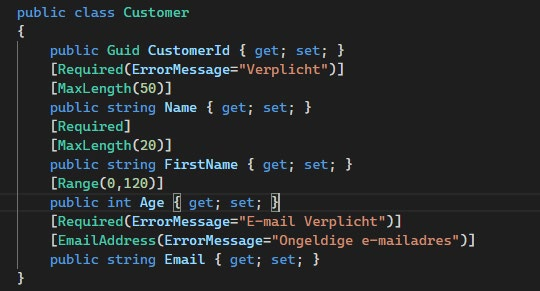
\includegraphics[width=0.5\textwidth]{validation-attributes.png}
    \caption{Validation attributes bij de properties}
\end{figure}


\begin{itemize}
    \item Attributen op de properties van het model
    \item Optioneel foutmelding meegeven aan attribuut, anders default waarde
    \item \textbf{[ApiController]} attribuut zorgt voor automatische validatie en HTTP Statuscode 400 indien niet OK
\end{itemize}

\begin{figure}[H]
    \centering
    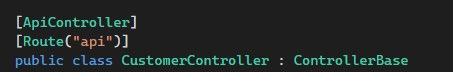
\includegraphics[width=0.5\textwidth]{validation-attributes2.png}
    \caption{ApiController boven de Controller-klasse}
\end{figure}

\begin{figure}[H]
    \centering
    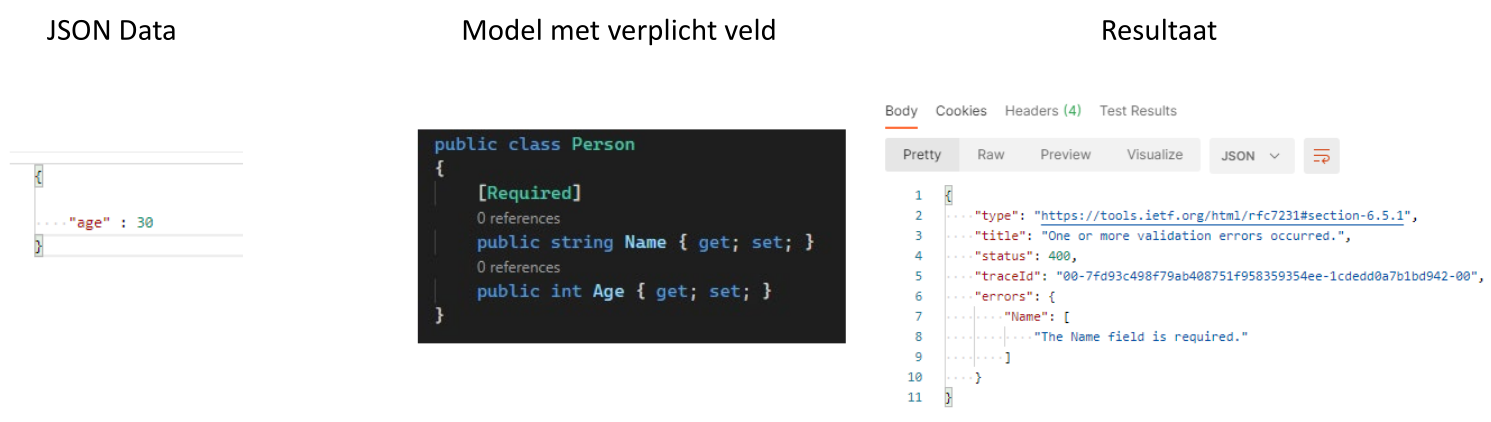
\includegraphics[width=0.9\textwidth]{validation-attributes-json.png}
    \caption{Je kan de error name veranderen: [Required(ErrorMessage="Sorry verplicht")]}
\end{figure}

\subsubsection{Ingebouwde attributen:}

\begin{itemize}
    \item {[CreditCard]} = creditcard formaat
    \item {[Compare]} = 2 properties moeten gelijk zijn in een model 
    \item {[EmailAddress]} = emailadres
    \item {[Phone]} = telefoonnummer
    \item {[Range]} = property value moet in een bepaald bereik zitten
    \item {[RegularExpression]}
    \item {[Required]} = vereist, niet leeg
    \item {[StringLength]} = maximum lengte
    \item {[Url]} = moet in URL-formaat zijn
\end{itemize}

\subsubsection{Custom Validation Attributes}

\begin{itemize}
    \item Zelf een Attribute maken: klasse erft van ValidationAttribute
    \item Override van methode ValidationResult
    \item In deze methode schrijven we de controle code
    \item Gebruiken in model [CustomerTypeAttribute]
\end{itemize}

\url{https://docs.microsoft.com/en-us/aspnet/core/mvc/models/validation?view=aspnetcore-5.0}

\begin{figure}[H]
    \centering
    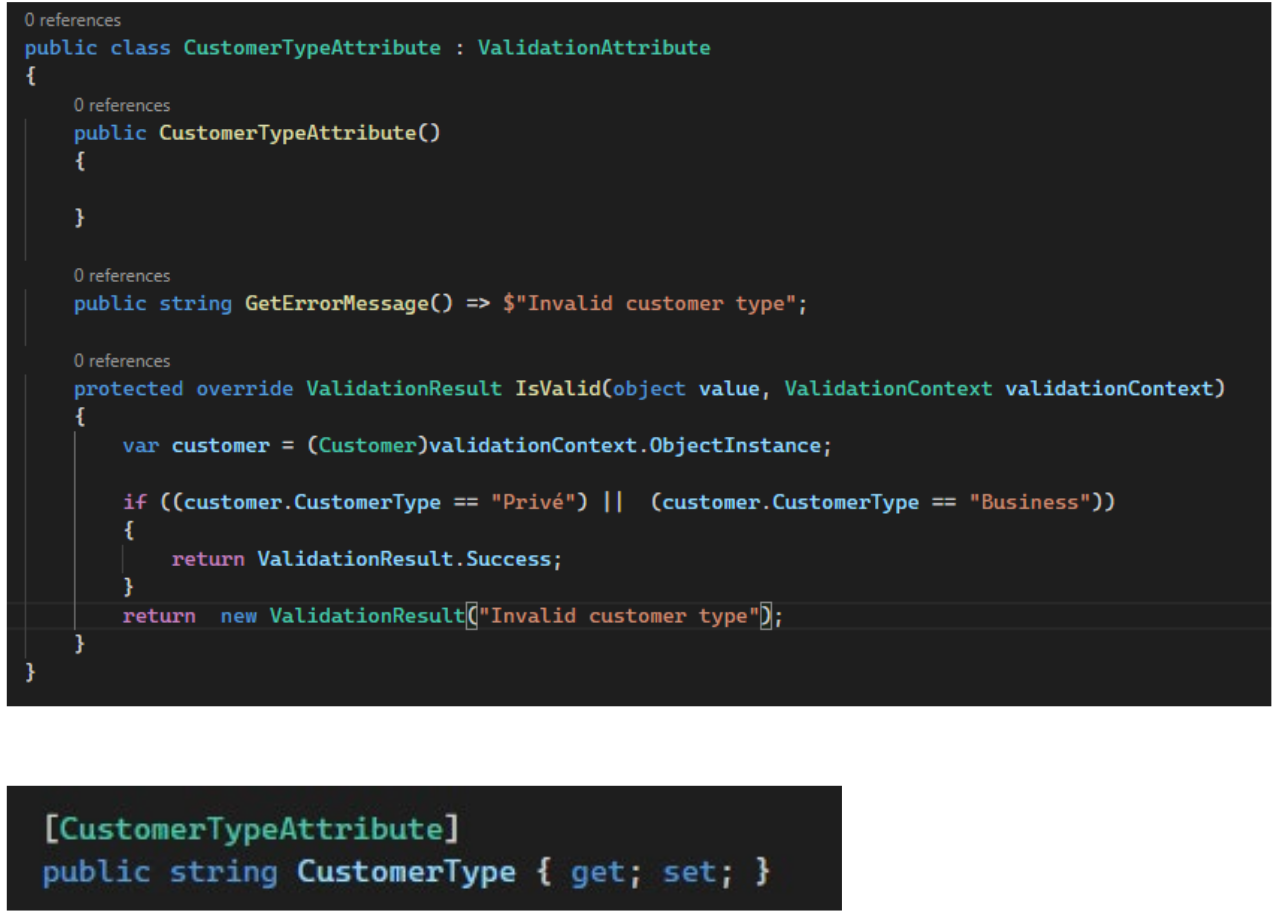
\includegraphics[width=0.65\textwidth]{validation-custom.png}
    \caption{}
\end{figure}

\subsection{QueryString}

= parameter in de url

\begin{itemize}
    \item Handig als we op verschillende manieren data wensen terug te keren zonder meerdere endpoints te maken
    \item \textcolor{red}{QueryString mogen \textbf{nooit} verplicht zijn}
    \item Gebruiken we vooral bij:
    \begin{itemize}
        \item Meegeven hoe we wensen te sorteren ?sort=asc
        \item Iets zoeken vb: ?q=zoekterm
        \item Iets in bepaalde taal opvragen vb: ?language=nl-BE
        \item Iets al dan niet includen of excluden
        \item Filters
    \end{itemize}
\end{itemize}

\subsubsection{Werking}

\begin{itemize}
    \item Waarde als parameter van de functie maar met default waarde vb: includeAddress
    \item IncludeAddress zit niet in de URL enkel CustomerId
    \item Geven we querystring niet mee dan zal includeAddress gelijk zijn aan false
\end{itemize}

\begin{figure}[H]
    \centering
    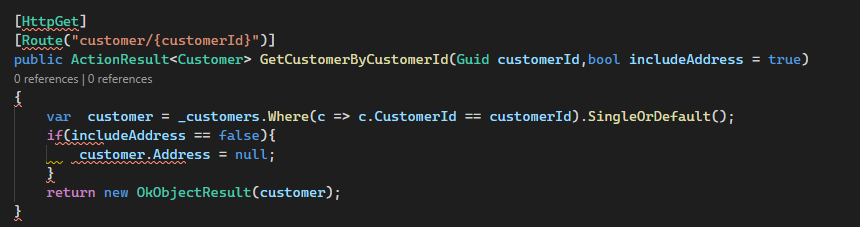
\includegraphics[width=0.6\textwidth]{querystring.png}
    \caption{}
\end{figure}

\subsection{DTO}

= Data Transfer Object

\begin{itemize}
    \item We kennen reeds models:
    \begin{itemize}
        \item POST = Omzetten van JSON naar C\# object 
        \item GET = Omzetten van C\# naar JSON object
    \end{itemize}
    \item Soms willen we niet alle data terugkeren: alleen terugsturen wat echt nodig is
    \item We voegen DTO klasse toe $\Rightarrow$ Alleen die properties sturen we terug
    \item Veel werk: alles manueel overzetten, bij nieuwe properties code aanpassen op verschillende plaatsen
\end{itemize}

\begin{figure}[H]
    \centering
    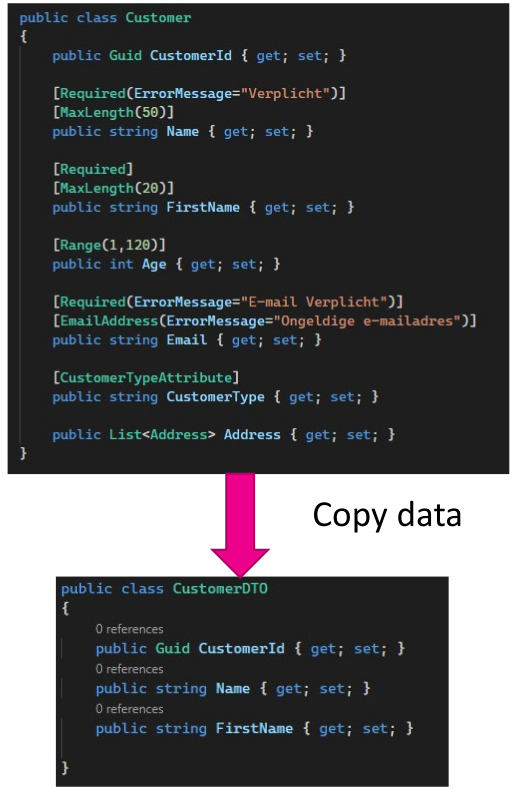
\includegraphics[width=0.4\textwidth]{dto.png}
    \caption{DTO moeten we manueel aanmaken en properties kopiëren}
\end{figure}

Oplossing:

\begin{itemize}
    \item een \textbf{mapper} gebruiken
    \item Nuget package die automatisch properties zal kopiëren tussen objecten
    \item Meest gebruikte in .NET wereld is \textbf{Automapper}
    \item \url{https://github.com/AutoMapper/AutoMapper}
\end{itemize}

\subsubsection{Werking}

\begin{figure}[H]
    \centering
    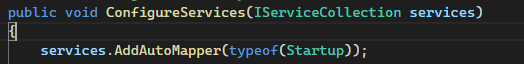
\includegraphics[width=0.5\textwidth]{dto-startup.png}
    \caption{In StartUp.cs: registreren van de AutoMapper service in WebAPI}
\end{figure}

\begin{figure}[H]
    \centering
    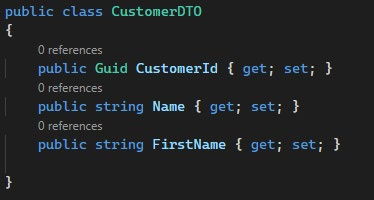
\includegraphics[width=0.5\textwidth]{dto-klasse.png}
    \caption{Klasse toevoegen in DTO-map, bv: CustomerDTO}
\end{figure}

\begin{figure}[H]
    \centering
    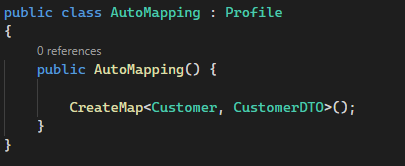
\includegraphics[width=0.5\textwidth]{dto-profile.png}
    \caption{DTO profile toevoegen, bv: AutoMapping.cs}
\end{figure}

In de AutoMapping klasse definiëren we de mapping tussen Customer en CustomerDTO

\begin{figure}[H]
    \centering
    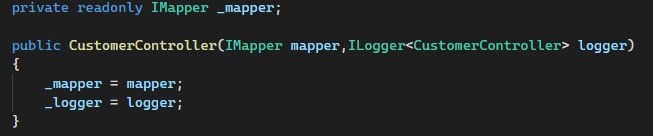
\includegraphics[width=0.5\textwidth]{dto-inject.png}
    \caption{We voeren de mapping uit door de automapper te injecteren in de controller (=dependency Injection)}
\end{figure}

\begin{figure}[H]
    \centering
    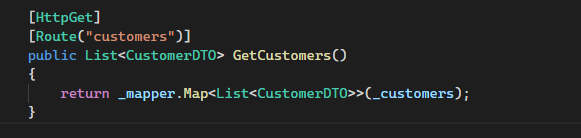
\includegraphics[width=0.5\textwidth]{dto-route.png}
    \caption{We passen de return value aan de controller en keren lijst van CustomerDTO terug. Via de Map-functie van de mapper zetten we deze om.}
\end{figure}


\subsection{Versioning}

\begin{itemize}
    \item Software veranderingen zijn er altijd, ook als software in productie is
    \item We moeten verschillende versies kunnen bouwen van onze API
    \item We moeten er rekening meehouden dat niet iedere client direct de nieuwe versie zal gebruiken $\Rightarrow$ oude versie blijven ondersteunen
    \item Hoe pakken we dit aan ?
    \item \textbf{Microsoft.AspNetCore.Mvc.Versioning} is de extra nuget package die we toevoegen
\end{itemize}

\subsubsection{Registreren bij services}

\begin{figure}[H]
    \centering
    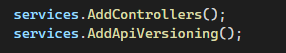
\includegraphics[width=0.5\textwidth]{versioning-services.png}
    \caption{Eerst registreren bij de services: \textbf{AddApiVersioning()}}
\end{figure}

\begin{figure}[H]
    \centering
    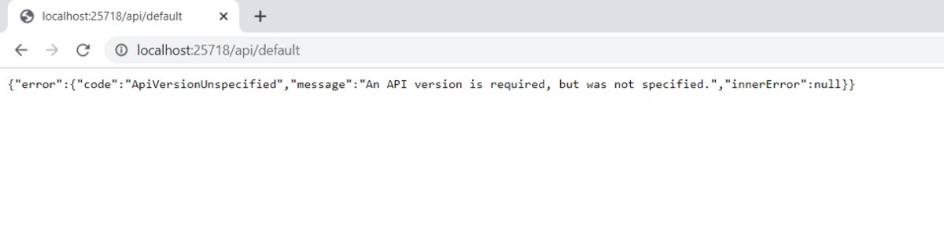
\includegraphics[width=0.5\textwidth]{versioning-browser.png}
    \caption{Alse we nu naar de endpoint surfen krijgen we een foutmelding dat we geen versie hebben meegegeven}
\end{figure}

\subsubsection{Configuratie}

\begin{itemize}
    \item We kunnen een default API versie instellen: \textbf{DefaultApiVersion}
    \item \textbf{AssumeDefaultVersionWhenUnspecified}: als er geen versie werd meegegeven, we veronderstellen dat dit default is
    \item We stellen ook in dat WebAPI de versie moet melden: \textbf{ReportApiVersion}
\end{itemize}

\begin{figure}[H]
    \centering
    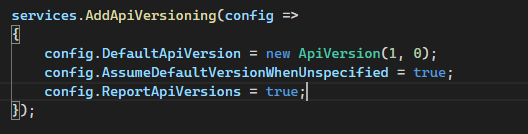
\includegraphics[width=0.5\textwidth]{versioning-addapiversioning.png}
    \caption{}
\end{figure}

\subsubsection{Controller attributes}

\begin{itemize}
    \item We stellen versies in op Controller niveau [ApiVersion]
    \item Verschillende versies zijn mogelijk
    \item Via [Deprecated] kunnen we melden dat een API zal verdwijnen op termijn
    \item Response header zal api-deprecated-versions terugkeren
\end{itemize}

\begin{figure}[H]
    \centering
    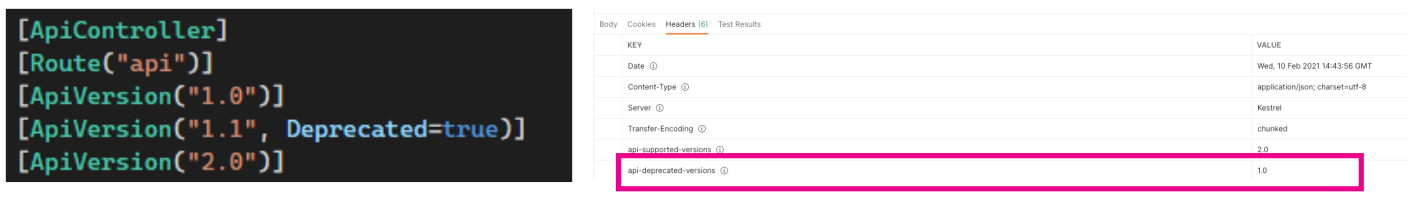
\includegraphics[width=0.5\textwidth]{versioning-deprecated.png}
    \caption{}
\end{figure}

\subsubsection{Endpoints mappen aan een specifieke versie}

\begin{figure}[H]
    \centering
    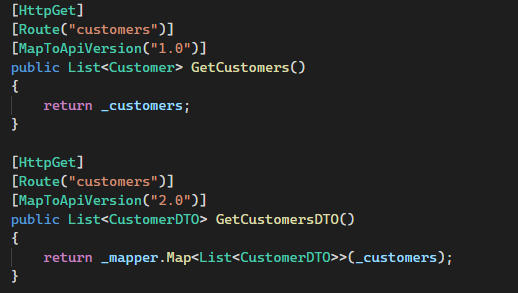
\includegraphics[width=0.5\textwidth]{versioning-maptoapiversion.png}
    \caption{[MapToApiVersion]}
\end{figure}

\subsubsection{Testen}

\begin{figure}[H]
    \centering
    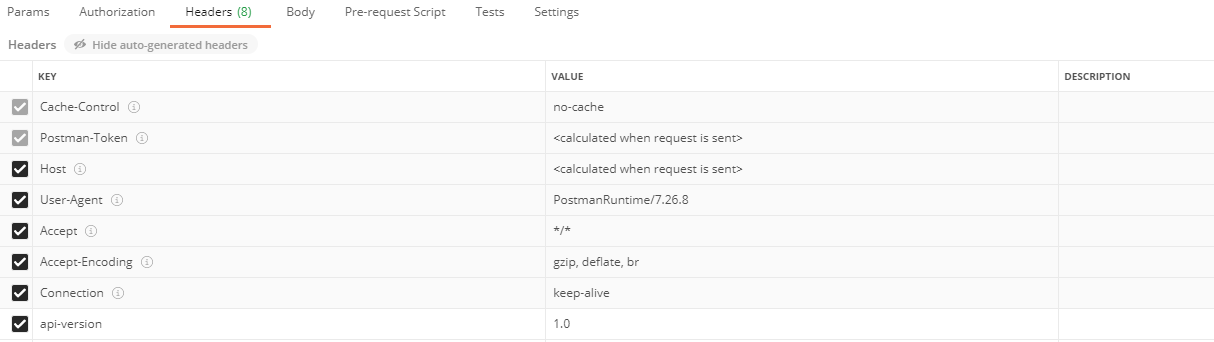
\includegraphics[width=0.5\textwidth]{versioning-httpheader.png}
    \caption{Via de HTTP header geven we de versie door}
\end{figure}

\subsection{Binary bestanden}

\begin{itemize}
    \item Naast JSON data moeten we soms ook met binary data werken
    \item Word, PDF, afbeeldingen, CSV \dots
    \item We moeten deze kunnen opladen naar een Web API
    \item We slaan deze dan op
    \begin{itemize}
        \item File system van de server (niet ok voor productie, wel om te testen)
        \item Blob Storage system op Azure (ok voor productie)
    \end{itemize}
\end{itemize}

\subsubsection{Werking}

\begin{itemize}
    \item We gebruiken HTTP Post
    \item List<IFromFile> bevat de bestanden
    \item Via for lus overlopen en wegschrijven naar C:\textbackslash Temp\textbackslash test.csv
    \item System.IO.File zorgt voor aanmaken file en wegschrijven data
\end{itemize}

\begin{figure}[H]
    \centering
    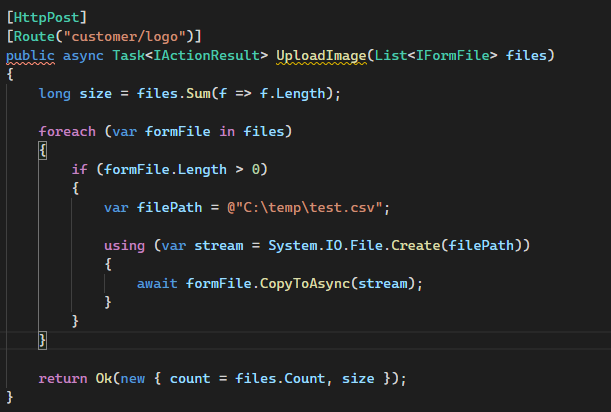
\includegraphics[width=0.5\textwidth]{binary-files.png}
    \caption{Werken met binary files}
\end{figure}

\subsubsection{Testen}

\begin{figure}[H]
    \centering
    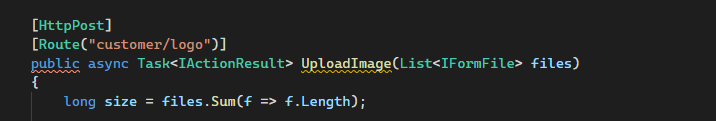
\includegraphics[width=0.6\textwidth]{binary-files-testing.png}
    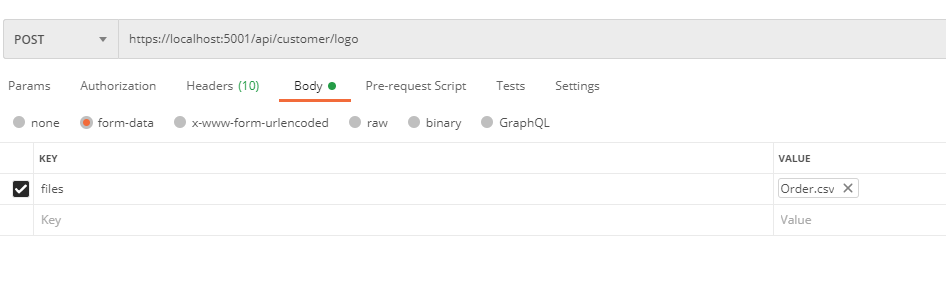
\includegraphics[width=0.6\textwidth]{binary-files-testing2.png}
    \caption{Testen via postman}
\end{figure}

\subsubsection{Bestanden downloaden}

\begin{itemize}
    \item We keren een FileResult terug
    \item Deze bevat:
    \begin{itemize}
        \item Stream met data
        \item mimeType = beschrijving file
        \item De naam van de file
    \end{itemize}
\end{itemize}

\begin{figure}[H]
    \centering
    \includegraphics[width=0.5\textwidth]{binary-files-download.png}
    \caption{Downloading files}
\end{figure}

\subsection{CSV files}

= Comma-Seperated Values

\begin{itemize}
    \item Veel gebruikt formaat zowel in wereld van AI, Administratieve apps,…
    \item Veel software kan overweg met dit formaat bv.: Excel (import/export)
    \item Is flat tekst formaat met een separator (komma, puntkomma, dubbelpunt, \dots)
    \item Seperator zal de data scheiden van elkaar
    \item Bevat meestal header, eerste rij in file
    \item In de wereld van AI veel gebruikt als formaat voor datasets
    \item Handig als we files kunnen genereren via Web API
\end{itemize}

\subsubsection{CSV Helper}

\begin{itemize}
    \item = Gratis en open source Nuget package voor lezen en schrijven van CSV files
    \item Goede documentatie en voorbeelden aanwezig
    \item \url{https://joshclose.github.io/CsvHelper/}
\end{itemize}

\subsubsection{Werking}

\begin{itemize}
    \item StreamWriter zal file wegschrijven
    \item CsvWriter zal CSV inhoud genereren
    \item Daarna zelfde procedure voor downloaden als andere file
    \item We slaan dus file eerst lokaal op, op de server
\end{itemize}

\begin{figure}[H]
    \centering
    \includegraphics[width=0.5\textwidth]{csv-werking.png}
    \caption{Voorbeeld CsvWriter}
\end{figure}

\subsection{Caching}

\begin{itemize}
    \item Applicatie sneller en schaalbaar maken
    \item We lezen niet altijd alle data uit de database
    \begin{itemize}
        \item Response is sneller $\Rightarrow$ database access (I/O in het algemeen is traag)
        \item Bv: lijst van landen: deze lijst zal niet veel wijzigen
    \end{itemize}
    \item 2 manieren in WebAPI:
    \begin{enumerate}
        \item Response caching
        \item Output caching
    \end{enumerate}
\end{itemize}

\subsubsection{Response Caching (HTTP Caching)}

\begin{itemize}
    \item HTTP Standaard RFC 7234: \url{https://tools.ietf.org/html/rfc7234}
    \item Hier gaan we de server zo weinig mogelijk inspannig vragen om een resultaat terug te keren
    \item We sturen de caching via de HTTP Headers
    \item Response caching zal niks opslaan op de server
    \begin{itemize}
        \item We slaan op bij de client of op proxy servers in het netwerk
        \item Server zal \textbf{Cache-Control} header toevoegen in response
        \item Private: client
        \item Public: op een proxy server
    \end{itemize}
\end{itemize}

\begin{figure}[H]
    \centering
    \includegraphics[width=0.5\textwidth]{caching-response-caching.png}
    \caption{Cache-Control in HTTP headers}
\end{figure}

\begin{figure}[H]
    \centering
    \includegraphics[width=0.5\textwidth]{caching-response-werking.png}
    \caption{In StartUp.cs moeten we een paar services registreren: services.AddResponseCaching()}
\end{figure}

\begin{figure}[H]
    \centering
    \includegraphics[width=0.5\textwidth]{caching-response-werking2.png}
    \caption{\textbf{app.UseResponseCaching()} toevoegen op de juiste plaats!}
\end{figure}

\begin{figure}[H]
    \centering
    \includegraphics[width=0.5\textwidth]{caching-response-werking3.png}
    \caption{Attribute [ResponseCache] toevoegen}
\end{figure}

ResponseCache attribuut

\begin{itemize}
    \item Duration in seconden
    \item Location: waar slaan we de cache op
    \begin{itemize}
        \item Any = public
        \item Client = private, geen caching op proxy
        \item None = geen cache
    \end{itemize}
\end{itemize}

\begin{figure}[H]
    \centering
    \includegraphics[width=0.5\textwidth]{caching-response-attribute.png}
    \caption{}
\end{figure}


\begin{itemize}
    \item \url{https://www.codeproject.com/Articles/1111260/Response-Caching-and-In-Memory-Caching-in-ASP-NET}
    \item \url{https://www.keycdn.com/blog/http-cache-headers}
\end{itemize}

\subsubsection{Output Caching}

\begin{itemize}
    \item We gaan resultaat bijhouden in een cache aan de server kant
    \item Memory intensief
    \item Schaalt niet altijd goed, zeker bij meerdere servers
    \item Oplossingen
    \begin{itemize}
        \item IMemoryCache, standaard in .NET core, eenvoudige maar geen scaling
        \item Redis
        \begin{itemize}
            \item Schaalt wel, maar duurder
            \item Extra service op Azure
            \item Zelf hosten als Docker container
        \end{itemize}
    \end{itemize}
\end{itemize}

\begin{figure}[H]
    \centering
    \includegraphics[width=0.4\textwidth]{caching-imemorycache.png}
    \includegraphics[width=0.7\textwidth]{caching-imemorycache2.png}
    \caption{IMemoryCache via services activeren in ConfigureServices}
\end{figure}

\begin{itemize}
    \item In de methode controleren via TryGetValue of de waarde aanwezig is
    \item Indien niet aanwezig: toevoegen via Set met als laatste parameter hoelang de waarde in de cache moet blijven
\end{itemize}

\begin{figure}[H]
    \centering
    \includegraphics[width=0.7\textwidth]{caching-output-trygetvalue.png}
    \caption{}
\end{figure}

\subsection{Wat moet je kennen?}

\begin{itemize}
    \item Wat is AutoMapper en hoe kan je dit gebruiken?
    \item Hoe werkt versioning in API's?
    \item Hoe kan je model validation doen?
    \item Wat is caching, waarom gebruiken we dit?
    \item Wat zijn de verschillende soorten caching in Web API?
    \item Hoe kan je best CSV bestanden verwerken?
    \item Hoe kan je binare bestanden opladen?
    \item Wanneer gebruiken we best querystrings en hoe?
\end{itemize}


\section{Docker \& Docker-compose}

\subsection{Waarom?}

\begin{itemize}
    \item Docker wil het mogelijk maken om software op ieder systeem te krijgen
    \item "If it runs on my computer, it will run on your computer"
    \item Microservices
    \item DevOps
    \item Resource usage
\end{itemize}

\subsection{What?}

\begin{itemize}
    \item Docker != container
    \item Docker = ecosysteem voor het creëren en draaien van containers
    \begin{itemize}
        \item Docker CLI
        \item Docker Engine
        \item Docker Image
        \item Docker Container
        \item Docker Hub
        \item Docker Compose
        \item Docker Swarm
    \end{itemize}
\end{itemize}

\subsection{Docker images}


\begin{itemize}
    \item = een snapshot van een filesystem
    \item Heeft een startup commando: executable die iets zal uitvoeren
    \item Heeft een gelaagde structuur (`layered structure')
\end{itemize}

Instantie van een image = container

\subsubsection{Image layers}

\begin{figure}[H]
    \centering
    \includegraphics[width=0.5\textwidth]{docker-image-layers.png}
    \caption{Image layers}
\end{figure}

\begin{itemize}
    \item De RUN, COPY, ADD commandos zullen allemaal een nieuwe read-only layer maken
    \item Top layer = container layer = de `writeable' layer
    \item Als je een container delete, zal alleen de container layer gedeletet worden
    \begin{itemize}
        \item Image zal blijven bestaan
        \item Om de data te behouden: gebruik persistente volumes (zie later)
    \end{itemize}
\end{itemize}

\subsection{Lightweight}

Docker images zijn heel klein in disk size, omdat:

\begin{itemize}
    \item De kernel van de host wordt gedeeld met Docker
    \item De container heeft geen OS nodig
    \item Om nog minder disk space te gebruiken $\Rightarrow$ layers delen
    \item Er zijn kleine community images:
    \begin{itemize}
        \item Alpine Linux
    \end{itemize}
\end{itemize}

\subsection{Microservices en Docker}

\begin{theorem}
    Microservices zijn een software development techniek die ervoor zorgen dat de 
    structuur van onze applicatie losgekoppeld wordt in verschillende kleine services
    die gekoppeld zijn aan elkaar
\end{theorem}

\begin{itemize}
    \item Lightweight
    \item Omgekeerde = monolithic architecture
    \begin{itemize}
        \item 1 server
        \item UI, Backend, Data Access Layer zit samen
    \end{itemize}
\end{itemize}

\begin{figure}[H]
    \centering
    \includegraphics[width=0.4\textwidth]{monolithic-vs-microservices.png}
    \caption{Bij microservices: elke service heeft zijn eigen server}
\end{figure}

\begin{figure}[H]
    \centering
    \includegraphics[width=0.6\textwidth]{monolithic-vs-microservices2.png}
    \caption{Links: containerized, monolithische applicatie. Rechts: Containerized microservices}
\end{figure}

Microservices != containerization (maar het is wel een logische stap)

\subsubsection{Demo}

\begin{figure}[H]
    \centering
    \includegraphics[width=0.5\textwidth]{microservices-demo.png}
    \caption{Een voorbeeld van een app die gebruik maakt van microservices en containers}
\end{figure}

\subsection{Docker basiscommando's}

\subsubsection{Images ophalen}

\begin{itemize}
    \item \textbf{Docker Hub}
    \item GCP Container Registry
    \item AWS Elastic Container Registry (ECR)
    \item Azure Container Registry (ACR)
    \item `Bring Your Own Registry' (binnekort bij Howest!)
    \item Er zijn ook private registries en repositories, waar je inloggegevens voor nodig hebt
    \item Standaard = Docker Hub
\end{itemize}

\textbf{Zoeken naar images}

\begin{itemize}
    \item hub.docker.com
    \item GitHub
    \item \dots
    \item docker search <keyword>
\end{itemize}

\textbf{Downloaden van images}

\begin{minted}{bash}
docker pull <image-naam>

# voorbeelden:
docker pull elasticsearch
docker pull nathansegers/some-custom-image
docker pull python:3.7-alpine
\end{minted}

\begin{itemize}
    \item Image tagging: een specifieke versie
    \item default = latest
    \item Belangrijk voor versioning (APIs)!
\end{itemize}

\subsubsection{Containers runnen}

\begin{minted}{bash}
# run een docker image
docker run <image-name> <alternative command>

docker create <image-name>
docker start <container-id>

# stop een container
docker stop (graceful) / docker kill (immediate)
# toon de huidige containers (--all toont ook de gestopte containers)
docker ps (--all)
\end{minted}

\subsubsection{Interactie \& logs}

$\Rightarrow$ geen GUI!

\begin{minted}{bash}
# interactieve terminal:
docker exec -it <container-id> <command>

# toon logs van een container
docker logs <container-id>

# verwijder alle gestopte containers, networken, images, build cache:
docker system prune
\end{minted}

\subsubsection{Containers builden}

\begin{minted}{bash}
# vergeet het puntje niet! dit betekent: onze huidige map
docker build .

# maak een image uit een bestaande container
docker commit -c <startup-command>
\end{minted}

\subsection{Dockerfile}

= Een bestand met commando's om een image te bouwen.

\begin{itemize}
    \item Volgorde is belangrijk!
    \item Gebruikt cache wanneer mogelijk (snellere builds)
    \item 
\end{itemize}

\begin{figure}[H]
    \centering
    \includegraphics[width=0.5\textwidth]{dockerfile.png}
    \caption{Voorbeeld Dockerfile}
\end{figure}

\begin{itemize}
    \item FROM: build image
    \item COPY: bestanden die we nodig hebben kopiëren
    \item RUN: commando's uitvoeren, programma's installeren
    \item WORKDIR: verander de huidige map
    \item ENTRYPOINT: startupcommando, met argumenten
\end{itemize}

\subsubsection{Dockerfile optimalisatie}

\begin{itemize}
    \item Herinner u: RUN, COPY, ADD voegt een nieuwe layer toe
    \item Wanneer we images builden, zullen de layers cache gebruikt worden
    \item We hebben in het vorig voorbeeld slechts 1 COPY commando gebruikt
    \item Stel dat we enkel de broncode van 1 bestand veranderd hebben:
    \begin{itemize}
        \item Dependencies zijn onveranderd
        \item Dependencies zullen toch opnieuw geinstalleerd worden, omdat de laag veranderd is
    \end{itemize}
\end{itemize}

Beter:

\begin{minted}{docker}
# packages installeren: als deze laag niet veranderd is, zal hij cache gebruiken
COPY *.csproj .
RUN dotnet restore

# pas daarna gaan we alle andere files kopiëren naar onze source map
COPY . .
# dan publiceren
RUN dotnet publish -c release -o /app
\end{minted}


\subsection{Docker Compose}

= meerdere containers runnen

\begin{itemize}
    \item In plaats van een dockercommando met enorm veel parameters:
    \begin{itemize}
        \item docker build .
        \item docker run -p 3000:3000 -v /app/node\_modules -v \$(pwd)\:\/app ca6cc440a6ef
    \end{itemize}
    \item Gebruiken we een .yaml bestand:
    \begin{itemize}
        \item docker-compose up --build
    \end{itemize}
\end{itemize}

\begin{minted}{yaml}
version: "3"
    services:
        web:
            build: .
            ports:
                - "3000:3000"
            volumes:
                - /app/node_modules
                - .:/app
\end{minted}

\begin{itemize}
    \item docker-compose.yml maakt het makkelijker om meerdere containers te draaien
    \item docker-compose.yml maakt het mogelijk om relaties tussen containers te leggen
\end{itemize}

\begin{figure}[H]
    \centering
    \includegraphics[width=0.5\textwidth]{docker-compose.png}
    \caption{Voorbeeld docker-compose.yml}
\end{figure}

\begin{minted}{bash}
# docker compose opstarten (of eerst builden en dan opstarten):
docker-compose up (--build)

# stoppen
docker-compose down
\end{minted}

\subsubsection{Docker Compose terminologie}

\begin{figure}[H]
    \centering
    \includegraphics[width=0.5\textwidth]{docker-compose2.png}
    \caption{Voorbeeld}
\end{figure}


In een docker-compose.yml bestand vind je volgende termen:

\begin{itemize}
    \item naam van de service
    \begin{itemize}
        \item In bovenstaand voorbeeld: `api'
    \end{itemize}
    \item image
    \begin{itemize}
        \item de image die we gebruiken voor deze service:
        \item nathansegers/custom-api:latest
    \end{itemize}
    \item build
    \begin{itemize}
        \item In welke map we gaan builden
        \item Relatief pad, ten opzichte van de context van het docker-compose.yml bestand
    \end{itemize}
    \item expose vs ports
    \begin{itemize}
        \item expose: 
        \begin{itemize}
            \item Opent een poort \textbf{binnen} het Docker netwerk
            \item Niet beschikbaar buiten docker
            \item Een applicatie die intern op poort 3306 draait, zal niet beschikbaar zijn op localhost:3306
            \item Geeft wel toegang aan andere services in hetzelfde netwerk
        \end{itemize}
        \item ports
        \begin{itemize}
            \item = interne port mapping
            \item Een applicatie die op poort 80 draait, zal beschikbaar zijn via localhost:5000
        \end{itemize}
    \end{itemize}
    \item networks
    \begin{itemize}
        \item We kunnen docker containers een netwerk geven zodat ze met elkaar kunnen communiceren
        \item Alle services zitten standaard in 1 netwerk
    \end{itemize}
    \item volumes
    \begin{itemize}
        \item Om bestanden te injecteren in een docker container
        \item Persistente storage
        \item Kan gedeeld worden met meerdere containers
        \item 2 manieren:
        \begin{enumerate}
            \item Named volumes
            \item Relatieve of absolute paden
        \end{enumerate}
        \begin{figure}[H]
            \centering
            \includegraphics[width=0.3\textwidth]{docker-volumes.png}
            \caption{Relatieve/absolute paden (boven) vs named volume (beneden)}
        \end{figure}
    \end{itemize}
    \item environments (.env)
    \begin{itemize}
        \item environment variables komen in dit bestand:
        \item connectionstrings
        \item ports
        \item databasenamen
        \item \dots
    \end{itemize}
    \item depends\_on
    \begin{itemize}
        \item Start de service na deze service(s)
        \item Hier: start de api nadat de db service is opgestart
        \item Dit is nodig als een service iets nodig heeft die een andere service eerst moet opstarten
    \end{itemize}
\end{itemize}



\subsection{Wat moet je kennen?}

\begin{itemize}
    \item Wat is docker? Waarom is het relevant voor ons?
    \item Wat zijn microservices?
    \item Hoe Dockerfiles schrijven
    \item De verschillende docker-compose termen
    \item Hoe communiceren tussen services in een Docker Network
\end{itemize}

\section{EF Core}

\subsection{Probleemstelling}

\begin{itemize}
    \item We gebruiken databases voor opslag van data
    \item Relationele databases is de standaard, meest gebruikt
    \item We gebruiken SQL in relationele databases voor INSERT, UPDATE, DELETE, \dots
    \item NoSQL databases wordenm meer en meer gebruikt:
    \begin{itemize}
        \item MongoDB
        \item CosmosDB
        \item ElasticSearch
    \end{itemize}
\end{itemize}

\subsubsection{\textcolor{red}{Niets fout} met SQL en relationele databases!}

\begin{itemize}
    \item Voordelen:
    \begin{itemize}
        \item SQL statements werken zeer snel
        \item Weinig nieuwe kennis nodig
    \end{itemize}
    \item Nadelen:
    \begin{itemize}
        \item Soms lastig om te onderhouden
        \item We schrijven SQL code \textbf{in} de C\# code
        \item Fouten zien we pas tijdens uitvoeren applicatie
    \end{itemize}
    \item Wanneer we SQL en NoSQL gebruiken binnen 1 applicatie $\Rightarrow$ meerdere APIs nodig
\end{itemize}

\subsubsection{Toch gebruiken we nog plain SQL}

\begin{itemize}
    \item Snelheid is nog altijd de beste, zeker als we stored procedures gebruiken die in de database draaien
    \item Super complexe queries en joins beter via SQL of Stored Procedure
    \item Bestaande toepassingen migreren naar EF Core is niet eenvoudig, deels migreren ook niet altijd
\end{itemize}

\subsection{EF Core}

= \textbf{Entity Framework Core}

\begin{itemize}
    \item Object Relationele Mapper (ORM)
    \item We mappen models (klassen) met tabellen in de database
    \item Via \textbf{LINQ} statements kunnen we operaties uitvoeren op de data
    \item We praten met de database via de \textbf{EF Context} $\Rightarrow$ speciale klasse die zorgt voor communicatie met de database
\end{itemize}

\begin{figure}[H]
    \centering
    \includegraphics[width=0.3\textwidth]{efcore-mapping.png}
    \caption{Database-tabel mappen naar een klasse}
\end{figure}

2 manieren van werken:

\begin{itemize}
    \item Database First
    \item Code first
\end{itemize}

\subsubsection{Database First}

\begin{itemize}
    \item We vertrekken van een bestaande database
    \item EF Core zal onze klassen genereren
    \item Vooral om bestaande toepassingen te moderniseren
\end{itemize}

\subsubsection{Code First}

\begin{itemize}
    \item Wij maken klassen (modellen)
    \item EF Core zal de database maken
\end{itemize}

Wij zien enkel Code First

\begin{figure}[H]
    \centering
    \includegraphics[width=0.5\textwidth]{database-code-first.png}
    \caption{Database-First vs Code-First}
\end{figure}

\subsection{EF Core installatie}

We moeten een \textbf{EF Core Provider} toevoegen aan het project:

\begin{itemize}
    \item Zorgt voor een onderliggende communicatie met de database
    \item Per database is er een provider
    \begin{itemize}
        \item Microsoft.EntityFrameworkCore.SqlServer (Azure)
        \item Microsoft.EntityFrameworkCore.Sqlite (Lokaal SQL Lite)
        \item Pomelo.EntityFrameworkCore.MySql (MySQL)
        \item CosmosDB $\Rightarrow$ NoSQL Support
        \item \url{https://docs.microsoft.com/en-us/ef/core/providers/?tabs=dotnet-core-cli}
    \end{itemize}
\end{itemize}

\begin{figure}[H]
    \centering
    \includegraphics[width=0.7\textwidth]{efcore-installatie-provider.png}
    \caption{}
\end{figure}

Toevoegen kan op 2 manieren:

\begin{itemize}
    \item VSCode > Command Palette > nu command > <provider naam>
    \item Via commandline in de map van je project
    \begin{itemize}
        \item dotnet add package Microsoft.EntityFrameworkCore.SqlServer
    \end{itemize}
\end{itemize}

Daarnaast moeten ook de EF tools op je systeem staan: dotnet tool install --global dotnet-ef

\subsection{Models}

Dit zijn klasses die onze database tables voorstellen. Een ID bepalen we door:

\begin{itemize}
    \item Het veld Id te noemen
    \item Naam van de klasse + Id $\Rightarrow$ BlogId
    \item Attribuut [Key]
    \item Dit zal autonummer worden in de database
\end{itemize}

\begin{figure}[H]
    \centering
    \includegraphics[width=0.7\textwidth]{efcore-model-id.png}
    \caption{3 manieren om een uniek ID aan te duiden}
\end{figure}

\subsubsection{Eén-op-veel-relaties}

\begin{figure}[H]
    \centering
    \includegraphics[width=0.6\textwidth]{efcore-model-eenopveel.png}
    \caption{Eén-op-veel-relaties}
\end{figure}


\begin{itemize}
    \item Blog bevat één of meerdere posts $\Rightarrow$ List<Post>
    \item Post kan slechts in één Blog voorkomen
    \item In de Post moeten we BlogId definiëren en kunnen we ook het Blog object zelf definiëren
    \item Dit noemen we een Navigation Property
\end{itemize}

\subsubsection{Enkele attributen}

\begin{minted}{csharp}
// Kolom zal in de database blog_id noemen en niet BlogId
[Column("blog_id")] 

// verplicht veld ook op database niveau
[Required]

// Provider zal dit meenemen bij database generatie, 
// veld in database zal ook max 500 karakters (nvarchar(500) zijn. 
// Anders is het nvarchar(max)
[MaxLength]  

// Provider zal dit instellen in databaseals decimal (5,2)
[Column(TypeName = "decimal(5,2)")]  

//
[Comment("database commentaar")]  
\end{minted}

\subsubsection{Fluent API}

\begin{itemize}
    \item We kunnen alle attributen ook via de Fluent API instellen
    \item Fluent API zijn functies die we kunnen aanroepen binnen OnModelCreating   
    \item Veel gebruikt voor configuratieinstallingen
    \item Ook enige optie als we \textbf{geen toegang} hebben tot de source code van de modellen:
    \begin{itemize}
        \item Dan kan je \textbf{geen attributen} plaatsen
        \item Enkel Fluent API mogelijk
    \end{itemize}
\end{itemize}

\begin{figure}[H]
    \centering
    \includegraphics[width=0.7\textwidth]{efcore-fluentapi.png}
    \caption{Fluent API}
\end{figure}

\subsection{EF Context}

(of DBContext)

\begin{itemize}
    \item Erft altijd van DBContext
    \item Klasse is verantwoordelijk voor de communicatie met de database via een sessie die deze opzet met de database
    \item We bepalen de tabellen, via DbSet
    \item We bepalen ook welke database we gebruiken via OnConfiguring waar we ConnectionString opgeven
    \item DbContext zal ook de relaties aanmaken en beheren
    \item Ook queries uitvoeren tov de database is een taak
\end{itemize}

\begin{figure}[H]
    \centering
    \includegraphics[width=0.6\textwidth]{efcore-dbcontext.png}
    \caption{BloggingContext erft van DBContext}
\end{figure}

\subsubsection{Aanmaken van de database en/of tabellen}

\begin{itemize}
    \item \textbf{Migrations} beschrijven in C\# code de aanmaak van de tabellen
    \item Bij iedere update moeten we een nieuw migratie aanmaken
    \item Er zal een map \textbf{Migrations} aangemaakt worden waarin alle veranderingen opgeslagen worden
\end{itemize}

\begin{minted}{bash}
# toevoegen van het ef tool om migraties te maken
dotnet add package MicrosoftEntityFrameworkCore.Design

# aanmaken van een migratie
dotnet ef migrations add <naam migratie>

# de aanpassingen uitvoeren:
dotnet ef database update
\end{minted}

\begin{itemize}
    \item Migratiebestanden bevatten C\# code die tabellen zal genereren in de database
    \item Wijzigt zelf \textbf{niks} in deze bestanden
    \item Bij iedere verandering in C\# code (nieuwe tabel, wijziging veld) moeten we een nieuwe migratie toevoegen: dotnet ef migrations add <naam migratie>
    \item Daarna moeten we de database updaten: dotnet ef database update
\end{itemize}

\subsection{Seeding}

= Opvullen van tabellen met \textbf{default} data (landen, postcodes, \dots)

\begin{itemize}
    \item Handig bij testen van software (unit en functional test)
    \item Seeding is onderdeel van migrations
    \begin{itemize}
        \item Eerst migrations uitvoeren
        \item Dan eventueel data seeding
    \end{itemize}
\end{itemize}

\subsubsection{In C\# code}

\begin{figure}[H]
    \centering
    \includegraphics[width=0.6\textwidth]{efcore-seeding.png}
    \caption{Seeding in C\#}
\end{figure}


\begin{itemize}
    \item Override de methode OnModelCreating
    \item Via modelBuilder $\Rightarrow$ hasData()
    \begin{itemize}
        \item Toevoegen entities
        \item Let op: autonummer moet je \textbf{WEL} invullen
    \end{itemize}
    \item Daarna zal deze code via migraties uitgevoerd worden
\end{itemize}

\subsection{Relations}

\subsubsection{One to Many}

Eén Blog heeft één of meerdere posts

\begin{itemize}
    \item Blog.BlogId = primary key
    \item Post.BlogId = foreign key
    \item Post.Blog = reference navigation property
    \item Blog.Post = collection navigation property
    \item Post.Blog = inverse navigation property
\end{itemize}

Relaties zullen default aangemaakt worden wanneer er navigation properties aanwezig zijn. 
EF Core zal dit detecteren en default zien als navigation properties

\begin{figure}[H]
    \centering
    \includegraphics[width=0.6\textwidth]{efcore-relations-onetomany.png}
    \caption{One to many}
\end{figure}

\subsubsection{One to One}

\begin{itemize}
    \item Automatische detectie van de navigation properties
    \item We kunnen dit ook configureren via de Fluent API
\end{itemize}

\begin{figure}[H]
    \centering
    \includegraphics[width=0.6\textwidth]{efcore-relations-onetoone1.png}
    \includegraphics[width=0.5\textwidth]{efcore-relations-onetoone2.png}
    \caption{}
\end{figure}

\subsubsection{Many to Many}

\begin{itemize}
    \item In beide modellen Collection navigation properties
    \item Automatische generatie van tussentabel
\end{itemize}

\begin{figure}[H]
    \centering
    \includegraphics[width=0.5\textwidth]{efcore-relations-manytomany.png}
    \caption{Many to Many}
\end{figure}

\subsection{SELECT, INSERT, UPDATE, DELETE}

\subsubsection{Hoe halen we records op (SELECT)?}

\begin{figure}[H]
    \centering
    \includegraphics[width=0.5\textwidth]{efcore-select.png}
    \caption{Records ophalen (HttpGet)}
\end{figure}

\begin{enumerate}
    \item BloggingContext aanmaken via \textbf{using} statement
    \item Via context.Blogs table aanspreken
    \item \textbf{ToListAsync} zal de query uitvoeren
\end{enumerate}



\begin{figure}[H]
    \centering
    \includegraphics[width=0.75\textwidth]{efcore-select2.png}
    \caption{SQL generatie door EF Core Context}
\end{figure}



\subsubsection{Hoe voegen we een record toe (INSERT)?}

\begin{figure}[H]
    \centering
    \includegraphics[width=0.5\textwidth]{efcore-insert.png}
    \caption{Records toevoegen (HttpPost)}
\end{figure}

\begin{enumerate}
    \item BloggingContext aanmaken via \textbf{using} statement
    \item Object toevoegen aan context.Blogs
    \item \textbf{SaveChangesAsync} aanroepen om weg te schrijven (asynchroon)
\end{enumerate}

\begin{figure}[H]
    \centering
    \includegraphics[width=0.75\textwidth]{efcore-insert2.png}
    \caption{SQL generatie door EF Core Context}
\end{figure}


\subsubsection{Hoe verwijderen we records (DELETE)?}

\begin{figure}[H]
    \centering
    \includegraphics[width=0.5\textwidth]{efcore-delete.png}
    \caption{Records deleten (HttpDelete)}
\end{figure}


\subsubsection{Hoe halen we records op (SELECT)?}

\begin{enumerate}
    \item BloggingContext aanmaken via \textbf{using} statement
    \item Eerst blog ophalen via de Linq Where clause
    \item We verwijderen de juiste blog uit de Context
    \item \textbf{SaveChangesAsync} zodat de database op de hoogte is
\end{enumerate}

\subsubsection{Toevoegen gerelateerde data (één op veel)}

Bv: hoe post toevoegen aan bestaande blog?

\begin{enumerate}
    \item Eerst blog opzoeken met zijn Posts
    \item Via Add methode voegen we een nieuwe Post toe en roepen we \textbf{SaveChangesAsync}
\end{enumerate}

\begin{figure}[H]
    \centering
    \includegraphics[width=0.5\textwidth]{efcore-insert-related.png}
    \caption{Gerelateerde data toevoegen (HttpPost met blogId parameter)}
\end{figure}


\begin{itemize}
    \item Via de using statement maken we de context aan
    \item Binnen de \{\} kunnen we objecten:
    \begin{itemize}
        \item manipuleren en wijzigen, 
        \item toevoegen
        \item verwijderen
    \end{itemize}
    \item De context zal deze veranderingen tracken
    \item Pas als we \textbf{SaveChangesAsync()} aanroepen zullen de veranderingen plaatsvinden in de database
\end{itemize}

\subsubsection{Hoe gerelateerde records ophalen}

\begin{figure}[H]
    \centering
    \includegraphics[width=0.5\textwidth]{efcore-select-related.png}
    \caption{Gerelateerde data ophalen (HttpGet blogs + de posts bij elke blog)}
\end{figure}


\begin{itemize}
    \item Via \textbf{Include} doen we een Join met een andere table
    \item Er zal \textbf{Exception} ontstaan bij serialisatie
    \begin{figure}[H]
        \centering
        \includegraphics[width=0.7\textwidth]{efcore-select-related2.png}
        \caption{}
    \end{figure}
    
    \item Oplossing: [JsonIgnore] toevoegen zodat serialisatie dit zal negeren
    \begin{figure}[H]
        \centering
        \includegraphics[width=0.5\textwidth]{efcore-select-related-jsonignore.png}
        \caption{}
    \end{figure}
\end{itemize}

\begin{figure}[H]
    \centering
    \includegraphics[width=0.5\textwidth]{efcore-select-related-result.png}
    \caption{Resultaat: JSON met voor elke blog alle posts van die blog}
\end{figure}


\subsection{Querying van data}

\begin{itemize}
    \item EF Core gebruikt \textbf{LINQ} (Language Integrated Query) om data op te halen uit de database
    \item We sturen LINQ query via Context naar de onderliggende database provider
    \item Deze database provider zal zorgen voor de vertaling naar SQL
    \item Je kan de SQL zien: toevoegen van Logger
\end{itemize}

\begin{figure}[H]
    \centering
    \includegraphics[width=0.5\textwidth]{efcore-querying-logger.png}
    \caption{Toevoegen van een Logger: in OnConfiguring}
\end{figure}

\subsubsection{Ophalen van alle Blogs \textit{zonder} Posts}

\begin{figure}[H]
    \centering
    \includegraphics[width=0.5\textwidth]{querying-select-zonder.png}
    \caption{}
\end{figure}


\begin{itemize}
    \item Context aanmaken
    \item Via Tabel Blogs methode ToListAsync() aanroepen
    \item ToListAsync() zal de query effectief uitvoeren, dit is het moment dat we naar de database gaan
\end{itemize}

\subsubsection{Ophalen van alle Blogs \textit{met} Posts}

\begin{itemize}
    \item Context aanmaken
    \item Via Tabel Blogs methode Include() aanroepen waar we meegeven welke gerelateerde tabel we willen mee ophalen
    \item b => b.Posts $\Rightarrow$ lambda expressie
    \item Op einde roepen we terug ToListAsync() om alles op te halen
    \item ToListAsync() zal de query effectief uitvoeren
\end{itemize}

\begin{figure}[H]
    \centering
    \includegraphics[width=0.5\textwidth]{querying-select-met.png}
    \caption{}
\end{figure}

\subsubsection{Ophalen van 1 specifiek item}

\begin{figure}[H]
    \centering
    \includegraphics[width=0.5\textwidth]{querying-select-1.png}
    \caption{Ophalen van 1 specifiek item}
\end{figure}

\begin{itemize}
    \item Via Where clause lambda meegeven: b => b.BlogId == blogId
    \textbf{\item SingleOrDefaultAsync()}
    \begin{itemize}
        \item query uitvoeren
        \item Single $\Rightarrow$ 1 resultaat
        \item OrDefault $\Rightarrow$ indien niks gevonden null terugkeren
    \end{itemize}
\end{itemize}

\subsubsection{Voorbeeld: comments van Post ophalen (3 tabellen diep)}

\begin{figure}[H]
    \centering
    \includegraphics[width=0.5\textwidth]{querying-voorbeeld.png}
    \caption{De comments van Post ophalen}
\end{figure}


\begin{itemize}
    \item Include zal eerst de Post ophalen
    \item ThenInclude zal voor iedere Post de comments ophalen
    \item ToListAsync() zal terug de query uitvoeren
\end{itemize}

\subsection{Generated Values}

\begin{figure}[H]
    \centering
    \includegraphics[width=0.3\textwidth]{efcore-generatedvalues.png}
    \caption{}
\end{figure}


\begin{itemize}
    \item Bij relationele databases hebben we de mogelijkheid om default waardes op te geven
    \item Handig voor bv Timestamps
    \item OnModelCreating override:
    \begin{itemize}
        \item Bij toevoegen Post, Blog of Comment
        \item Autmoatische DateTime.Now() in veld `Created'
    \end{itemize}
\end{itemize}

\subsection{Extra info}

\begin{itemize}
    \item \url{https://www.entityframeworktutorial.net/efcore/entity-framework-core.aspx}
    \item \url{https://docs.microsoft.com/en-us/ef/core/}
\end{itemize}

\subsubsection{Wat moet je zeker kennen?}

\begin{itemize}
    \item Wat en waarom EF Core?
    \item Opbouw $\Rightarrow$ model, migrations
    \item Welke attributen zijn er?
    \item De commands om migraties te maken en updates te doen
    \item Hoe kan je data opvragen?
    \item Hoe zitten de relaties in elkaar?
\end{itemize}

\section{Services \& Repositories}

\subsection{Probleemstelling}

\subsubsection{Wat hebben we reeds gezien?}

\begin{itemize}
    \item We kunnen API's maken
    \item We kunnen deze hosten in Docker containers
    \item We kunnen wegschrijven naar databases die ook in Docker draaien
\end{itemize}

\subsubsection{Probleemstelling}

\begin{itemize}
    \item Weinig structuur in onze code
    \begin{itemize}
        \item Controller bevat database code (EF Core)
        \begin{itemize}
            \item We halen data op in de controller
            \item We voegen data in de database vanuit de controller
            \item Weinig herbruikbaarheid van code mogelijk
        \end{itemize}
        \item Geen vaste structuur waar o.a. business logica komt, bv: prijsberekening
        \begin{itemize}
            \item Stel dat we de prijs meoten berekenen, dan gaan we dat tot nu doen in de controller zelf
        \end{itemize}
    \end{itemize}
    \item Controllers moeten zo clean mogelijk zijn
    \begin{itemize}
        \item Geen logica in controller methode
        \item Enkel validatie en doorverwijzing naar andere laag
    \end{itemize}
\end{itemize}

\subsubsection{Oplossing: Design Patterns}

We introduceren \textbf{Design Patterns}:

\begin{itemize}
    \item We gaan meer structuur geven aan onze applicatie
    \item Zorgt voor meer betrouwbare code
    \item Makkelijker voor onderhoud en aanpassingen
    \item Nieuwe teamleden zullen sneller weg vinden in de code
    \item Patterns zijn \textbf{niet} verbonden aan een taal (zowel in C\#, Python, \dots)
\end{itemize}

Opgepast:

\begin{itemize}
    \item Design Patterns lossen niet alles op
    \item introduceren soms meer complexiteit en meer werk
\end{itemize}

\subsubsection{Repository \& Service pattern}

\begin{figure}[H]
    \centering
    \includegraphics[width=0.25\textwidth]{repository-service-pattern.png}
    \caption{}
\end{figure}

We introduceren Repository \& Service pattern

\begin{itemize}
    \item Controller zal praten met Service laag
    \begin{itemize}
        \item Service laag (Business layer0 bevat de Business logica)
        \item Business logica is:
        \begin{itemize}
            \item Berekeningen, beslissingen
            \item Ophalen van data uit de database om beslissingen te nemen
        \end{itemize}
    \end{itemize}
    \item Service laag zal praten met Repository laag
    \begin{itemize}
        \item Repository bevat code om met database te spreken
        \item Hier zullen we onze LINQ queries schrijven
    \end{itemize}
    \item Er zijn veel andere patterns, bv: Mediator pattern \url{https://www.dofactory.com/net/mediator-design-pattern}
\end{itemize}

\subsection{Repositories}

\begin{itemize}
    \item Bevat enkel de code om database operaties uit te voeren $\Rightarrow$ single responsibility principe
    \item We proberen per tabel een repository te maken, maar je kan/mag hier van afwijken
    \item Via de Context voeren we LINQ queries uit
    \item Context zal via \textbf{Dependency Injection (DI)} aanspreekbaar zijn in de repository
\end{itemize}

\subsubsection{In de praktijk}

\begin{figure}[H]
    \centering
    \includegraphics[width=0.5\textwidth]{repositories-1.png}
\end{figure}

\begin{itemize}
    \item Map Repositories in project
    \item We voegen VaccinTypeRepository.cs toe
    \item In deze class gaan we onze methode schrijven, bv: GetVaccins()
\end{itemize}

\subsubsection{Probleem}

\begin{itemize}
    \item We maken context aan in de repository
    \item We moeten null parameters doorgeven
    \item Hierdoor is RegistrationContext \textbf{tightly coupled} met VaccinTypeRepository
    \item Ze kunnen \textbf{niet} zonder elkaar bestaan
    \item Dit is niet zo goed naar herbruikbaarheid
    \item Zeer lastig om te testen
\end{itemize}

\begin{figure}[H]
    \centering
    \includegraphics[width=0.5\textwidth]{repositories-2.png}
    \caption{}
\end{figure}


\subsubsection{Oplossing}

\begin{itemize}
    \item We moeten de context \textbf{loose coupled} maken
    \item Ze moeten elkaar begrijpen, maar ze mogen niet afhankelijk zijn van elkaar
    \item Nu gaan we er vanuit dat RegistrationContext zal verwijzen naar onze Docker SQL server
    \item Bij testen willen we een andere database gebruiken $\Rightarrow$ in deze opstelling lastig
    \item We wensen dus flexibiliteit
\end{itemize}

\begin{figure}[H]
    \centering
    \includegraphics[width=0.5\textwidth]{repositories-3.png}
    \caption{Abstractie van de RegistrationContext: we maken een C\# interface}
\end{figure}

\begin{itemize}
    \item We maken abstractie van de RegistrationContext
    \item We gaan bepalen welke methodes er aanwezig zijn, maar niet wat ze moeten doen
    \item We introduceren een C\# interface
\end{itemize}

\begin{figure}[H]
    \centering
    \includegraphics[width=0.5\textwidth]{repositories-4.png}
    \caption{}
\end{figure}

\begin{itemize}
    \item De interface zal specificeren welke methodes er aanwezig zijn
    \item Iedere klasse die de interface gaat implementeren kan zijn eigen kan dan eigen context voorzien
    \item We gaan dit ook doen voor Repositories \& Services. Altijd een interface voorzien
\end{itemize}

Hoe moeten we deze nu gebruiken?

\begin{itemize}
    \item Hoe moet de Repository de RegistrationContext gebruiken ?
    \item Hoe moet de Controller de Repository gebruiken ?
\end{itemize}

$\Rightarrow$ Dependency Injection

\subsection{Dependency Injection (DI)}

\begin{itemize}
    \item We gebruiken dit reeds enkele weken
    \item Alles in ASP.NET WebAPI is DI based
    \begin{itemize}
        \item Swagger gebruikt DI
        \item services.AddControllers() doet dit ook
    \end{itemize}
\end{itemize}

\subsubsection{Wat is dat nu eigenlijk}

\begin{itemize}
    \item Dit is terug een Design pattern
    \item Doelstelling is Inversion of Control (IoC) bekomen
    \begin{itemize}
        \item Het aanmaken van objecten gaan we uit handen geven aan een \textbf{IoC container}
        \item We zijn gewoon om VaccinTypeRepository p = new VaccinTypeRepository() te schrijven
        \item De IoC container zal dit voor ons doen achter de schermen
        \item Via DI zal dit object beschikbaar zijn als we het nodig hebben
        \item Indien je niet tevreden bent kan je de ASP.NET IoC Container uitpluggen en zelf maken
    \end{itemize}
\end{itemize}

\subsubsection{Werking}

\begin{itemize}
    \item De objecten die we wensen te gebruiken via DI moeten we registreren in de IoC container
    \item Dit zal gebeuren in Startup.cs in de methode ConfigureServices
    \item Er zijn 3 manieren van registratie:
    \begin{enumerate}
        \item AddTransient
        \begin{itemize}
            \item Bij iedere HTTP request zal er een nieuwe instantie gemaakt worden van het object
            \item Tijdens hetzelfde request ook een nieuw object indien nodig
        \end{itemize}
        \item AddScoped
        \begin{itemize}
            \item Bij iedere HTTP request een nieuw object
            \item Maar tijdens hetzelfde request zal het object hergebruikt worden
        \end{itemize}
        \item AddSingleton
        \begin{itemize}
            \item Bij de eerste request zal er object gemaakt worden
            \item Daarna zal hetzelfde object gebruikt worden als het nog eens nodig is
            \item Ook over verschillende users $\Rightarrow$ oppassen
        \end{itemize}
    \end{enumerate}
\end{itemize}


\begin{figure}[H]
    \centering
    \includegraphics[width=0.5\textwidth]{dependency-injection-registratie.png}
    \caption{\url{https://www.c-sharpcorner.com/article/understanding-addtransient-vs-addscoped-vs-addsingleton-in-asp-net-core/}}
\end{figure}

\subsubsection{In de praktijk}

We registreren in Startup.cs in de IoC Container de objecten RegistrationContext en VaccinTypeRepository

Als er nu ergens in onze applicatie een IRegistrationContext of IVaccinTyperepository interface nodig is, 
dan zal er een object gemaakt van hun respectievelijk type RegistrationContext en VaccinTypeRepository:

\begin{figure}[H]
    \centering
    \includegraphics[width=0.75\textwidth]{dependency-injection-1.png}
    \caption{}
\end{figure}

\begin{itemize}
    \item In onze VaccinTypeRepository hebben we de RegistrationContext nodig want anders kunnen we niet praten met de database
    \item We maken gebruik van constructor injection om een instantie van RegistrationContext binnen te brengen in onze VaccinTypeRepository
    \item De IoC container van ASP.NET Core heeft voor IRegistrationContext een RegistrationContext object geregistreerd in Startup.cs
    \item Bij het uitvoeren van het project ziet .NET dat er een IRegistrationContext nodig is bij VaccinTypeRepository. ASP.NET vraagt aan de IoC container een object waar de interface IRegistrationContext voor is geregistreerd en zal dit binnen brengen via de constructor.
\end{itemize}

\begin{figure}[H]
    \centering
    \includegraphics[width=0.5\textwidth]{dependency-injection-2.png}
    \caption{}
\end{figure}

\begin{figure}[H]
    \centering
    \includegraphics[width=0.9\textwidth]{dependency-injection-3.png}
    \caption{Stel dat we IRegistrationContext niet geregistreerd hebben in de Startup.cs: veel gemaakt error!}
\end{figure}

\begin{figure}[H]
    \centering
    \includegraphics[width=0.5\textwidth]{dependency-injection-4.png}
    \caption{We passen nu ook onze Controller aan en injecteren de repository in de Controller}
\end{figure}

\subsection{Services}

De service layer bevat:

\begin{itemize}
    \item Business Logica
    \begin{itemize}
        \item Prijsberekening
        \item Procedures
        \item Andere services aanroepen, vb mail sturen
    \end{itemize}
    \item Aanroepen naar databas
    \begin{itemize}
        \item Soms is het gewoon doorgeven van method calls
        \item Veel overhead code soms
    \end{itemize}
\end{itemize}

We gaan niet voor iedere Repository een service maken, de service zal meer op functioneel niveau gaan groeperen, bijvoorbeeld:

\begin{itemize}
    \item PriceService
    \begin{itemize}
        \item ProductRepository
        \item DiscountRepository
        \item \dots
    \end{itemize}
    \item OrderService
    \begin{itemize}
        \item ProductRepository
        \item DiscountRepository
        \item EmailService $\Rightarrow$ service aanroepen vanuit andere services
    \end{itemize}
\end{itemize}

\subsubsection{In de praktijk}

\begin{itemize}
    \item Mapje Services in het project
    \item Klasse VaccinationService
    \item We injecteren de IVaccinTyperepository in de service
    \item Daarna kunnen we de repository gebruiken
\end{itemize}

\begin{figure}[H]
    \centering
    \includegraphics[width=0.5\textwidth]{services-1.png}
    \caption{}
\end{figure}

Nu moeten we de service registreren zodat we deze kunnen gebruiken:

\begin{figure}[H]
    \centering
    \includegraphics[width=0.7\textwidth]{services-2.png}
    \caption{Registratie VaccinationService}
\end{figure}

In de controller injecteren we nu de IVaccinationService en niet meer de Repository

\begin{figure}[H]
    \centering
    \includegraphics[width=0.5\textwidth]{services-3.png}
    \caption{Injectie IVaccinationService}
\end{figure}

\subsection{Wat is belangrijk?}

\begin{itemize}
    \item Wat is doel van repository en services?
    \item Wat is DI en IoC?
    \item Waarom interfaces nodig?
    \item Welke zijn de drie manieren om services te registeren in .NET Core?
\end{itemize}


\end{document}